\documentclass[prl,reprint]{revtex4-1}
%\documentclass[12pt]{article}

\usepackage{amsmath}
\usepackage{amsfonts}

\usepackage{graphicx}
\usepackage{subcaption}


\begin{document}


\title{Choosing Appropriate Metrics for Diffusion Maps Analysis: A Chemotaxis Case Study}

\author{Carmeline J. Dsilva}
\email{cdsilva@princeton.edu}
\affiliation{Department of Chemical and Biological Engineering, Princeton University, Princeton, NJ, 08544}

\author{Ronen Talmon}
\email{ronen.talmon@yale.edu}
\affiliation{Department of Mathematics, Yale University, New Haven, CT, 06520}

\author{Ronald R. Coifman}
\email{coifman@math.yale.edu}
\affiliation{Department of Mathematics, Yale University, New Haven, CT, 06520}

\author{Ioannis G. Kevrekidis}
\email{yannis@princeton.edu}
\affiliation{Department of Chemical and Biological Engineering, Princeton University, Princeton, NJ, 08544}
\affiliation{Program in Applied and Computational Mathematics, Princeton University, Princeton, NJ, 08544}

\date{\today}

\begin{abstract}

We have a simulation of the dynamical system that is governed basically by a single parameter,­ the rate of switching.
 %
 Depending of the value of this parameter, this system dynamics range between heat equation dynamics and wave equation dynamics. 
 %
 In the heat equation dynamics, the initial conditions play very little role and the system dynamics over time are dominant. 
 %
 In the wave equation dynamics, the initial conditions play a significant role and the dynamics over time are less important.
 %
We demonstrate that an essential component of our analysis is working with the right observers (histograms/ensumble rather than a single position of a particle) and with the right metric between those observers (EMD).
%
We demonstrate that we recover the right factors that control the dynamical system, depending on the mode (In heat eq. mode ­ first recover the temporal dynamics, second the initial conditions; In wave eq. mode ­ first recover the initial conditions, second the temporal dynamics). In particular, these two components have a completely different ``nature". For example, in this case, one parameter (initial condition) is governing the entire trajectory and the other parameter (dynamics) is governing the ``step­--by­--step" time evolution (within each trajectory).
\end{abstract}

\keywords{diffusion maps, earth mover's distance, histograms}

\maketitle

\section{Introduction} 
 
In dynamical systems, it is often essential to detect changes in the characteristic behavior of a system.
%
Methods such as bifurcation analysis, etc., have been developed with such problems in mind. 

We will demonstrate how we can use data mining techniques (diffusion maps \cite{coifman2005geometric}) to {\em automatically} detect changes in a system's behavior.
%
We will illustrate our dynamics through a model problem arising in studies of cellular chemotaxis \cite{othmer2000diffusion}.
%
In our methods, it will be esseintial 


\section{Problem formualtion}

\subsection{Chemotaxis ``story''} 

We look at a stochastic velocity jump process that arises in models of chemotaxis \cite{othmer2000diffusion}.
%
Chemotaxis is the movement of cells (such as bacteria) that is regulated by extracellular sensed signals.
%
Such signals allow cells to accomplish tasks such as finding food and navigating away from toxins.
%
Biologists are interested in the dynamics of cellular movement and dispersal, and several models have been proposed \cite{othmer1988models, codling2008random}.
%
We will look at a velocty jump process model of these dynamics.
%
In such models, each cell is initialized with a position and a velocity, and the dynamics of each cell are governed by a stochastic process.
%
In a velocity jump process, at random times, cells will ``turn around'' and switch their velocity (this turning is thought to be driven by extracellular signals from food or toxins). 
%
We will analyze the dynamics of collections of such cells/particles. 

\subsection{Stochastic particles}

Assume we have a collection of $N$ particles, each of which has a position and velocity. 
%
Let $x_i(t)$ and $v_i(t)$ denote the position and velocity, respectively, of particle $i$ at time $t$.
%
The velocity of each particle is either $\pm s$, where $s$ is the speed. 
%
We initialize the particles such that
\begin{equation}
\begin{aligned}
x_i(0) & = 0 \\
\mathbb{P} \{ v_i(0) = +s \} & = p
\end{aligned}
\end{equation}
where $p$ is some probability.
%
The velocity of each particle randomly switches between $\pm s$ following an (independent) Poisson process with rate $\lambda$.
%
Note that each particle has its own ``clock" (Poisson process).

\subsection{Partial differential equations}

Let $X_{p, \lambda, s}(t)$ denote the vector of positions of the particles at time $t$ with initial right probability $p$, switching rate $\lambda$, and speed $s$.

Let $\rho(x, t)$ denote the probability density of the particles, and let $\rho^-(x, t)$ and $\rho^+(x, t)$ denote the probability density of the left and right moving particles, respectively.
%
It can be shown that, as $n \rightarrow \infty$, $\rho(x, t)$ obeys the following set of partial differential equations (PDEs)
\begin{equation} \label{eqn:coupled_pdes}
\begin{aligned}
\frac{\partial \rho^+}{\partial t} + s \frac{\partial \rho^+}{\partial x} & = -\lambda \rho^+ +\lambda \rho^- \\
\frac{\partial \rho^-}{\partial t} - s \frac{\partial \rho^-}{\partial x} & = \lambda \rho^+ -\lambda \rho^- 
\end{aligned}
\end{equation}
%
Alternatively, \eqref{eqn:coupled_pdes} can be written as one, second--order PDE
\begin{equation} \label{eq:second_order_pde}
\frac{\partial^2 \rho}{\partial t^2} + 2 \lambda \frac{\partial \rho}{\partial t} = s^2 \frac{\partial ^2 \rho}{\partial x^2}
\end{equation}
%
We assume that $s^2/\lambda = D$ is constant.
%
Therefore, the dynamics are governed {\em only} by a single parameter $\lambda$.

\subsection{Asymptotic mode analysis}  \label{subsec:mode_analysis}

We will consider two regimes of simulation.
%
When $\lambda \rightarrow 0$, one can see that the right-hand side of \eqref{eqn:coupled_pdes} tends to 0. 
%
Therefore, \eqref{eqn:coupled_pdes} becomes two uncoupled wave equations.
%
Alternatively, in this regime, in the limit the second order equation \eqref{eq:second_order_pde} becomes 
\[
\frac{\partial^2 \rho}{\partial t^2} = s^2 \frac{\partial ^2 \rho}{\partial x^2},
\]
i.e., the second order wave equation.

Dividing \eqref{eq:second_order_pde} by $\lambda > 0$ yields
\[
\frac{1}{\lambda} \frac{\partial^2 \rho}{\partial t^2} + 2 \frac{\partial \rho}{\partial t} = D \frac{\partial ^2 \rho}{\partial x^2}
\]
When $\lambda \rightarrow \infty$, \eqref{eq:second_order_pde} approaches the heat equation
\[
2 \frac{\partial \rho}{\partial t} = D \frac{\partial ^2 \rho}{\partial x^2}
\]
 
\section{Methods and Analysis}

\subsection{Diffusion maps}

We will use diffusion maps \cite{coifman2005geometric} to analyze the data from our stichastic simulations.
%
Diffusion maps is a nonlinear dimensionality reduction technique.
%
In our simulations, although the data is very high--dimensional (each data point contains the positions of all $N$ particles), there are only two important parameters ($p$ and $t$) that determine the current state of the system.

Assume we have data points $z_1, z_2, \dots, z_m \in \mathbb{R}^p$, but that these data points lie on a $d$-dimensional, nonlinear manifold, with $d \ll p$. 
%
We want to uncover a $d$-dimensional parameterization of the points $x_1, \dots, x_m$.
%
We first construct the matrix $W \in \mathbb{R}^{m \times m}$, with
\begin{equation} \label{eq:W}
W_{ij} = \exp \left( -\frac{\|z_i - z_j \|^2}{\epsilon^2} \right)
\end{equation}
where $\| \cdot \|$ denotes the appropriate norm for the data (we will discuss the choice of norm in the following section), and $\epsilon$ is a characteristic distance between the data points.
%
We then construct the diaganol matrix $D \in \mathbb{R}^{m \times m}$, with $D_{ii} = \sum_j W_{ij}$, and then the matrix $A$, defined as
\begin{equation}
A = D^{-1} W.
\end{equation}
%
We then compute the eigenvalues $\lambda_1, \lambda_2, \dots, \lambda_m$ and eignevalues $\phi_1, \phi_2, \dots, \phi_m$ and order them such that $|\lambda_1| \ge |\lambda_2| \ge \dots \ge |\lambda_m|$. 
%
Note that the matrix $A$ is row--stochastic ($\sum_j A_{ij} = 1$), which implies $\lambda_1 = 1$ and $\phi_1$ is a constant vector.
%
The next few eigenvectors $\phi_2, \phi_3, \dots$ give us the embedding coordinates for our data, such that $\phi_j(i)$ gives us the $j^{th}$ embedding coordinate for $x_i$.

As we can see from the analysis in \ref{subsec:mode_analysis}, the ``important'' quantity to describe the dynamics is not the positoin of each particle, but rather the probability density of the particles.
%
We will empirically estimate the probability density for each timepoint by computing the histogram of the particle positions. 
%
Therefore, $z_i \in \mathbb{R}^p$ will be the histogram of $x_1, x_2, \dots, x_N$ into $p$ bins.

\subsection{Earth mover's distance}

The {\em essential} requirement for diffusion maps is having an appropriate distance metric between data points to compute $W$ in \ref{eq:W}.
%
Often, one uses the Euclidean distance between data points;
however, for histograms which approximate a probability density, the Euclidean distance can often be misleading.
%
For example, the distance between two uniform distributions with finite, non-overlapping support will always be the same, {\em independent} of the distances between the support intervals.
%
Intuitively, we would want/expect two distributions whose supports are close to be closer (in norm) than two distributions whose supports are very far from each other.

We therefore use the earth mover's distance (EMD) \cite{rubner2000earth} as the metric between our histograms.
%
Conceptually, EMD measures how much ``work'' it takes to transform one probability density into another.
%
It therefore not only considers where the densities are incosistent, but how far apart they are.

Although the brute--force computation of the EMD between two histograms is computationally expensive, there has been a plethora of work in developing efficient algorithms for the computation of EMD \cite{...}.
%
%TODO: we need to pay a special attention to the implementation of the EMD. We need to make it cleat that this distance can be very efficiently implemented  and therefore it is suitable for the practical uses and algorithm that we propose here as a viable tool for dynamical system analysis.
%
We use the EMD implementation from \cite{Pele-eccv2008, Pele-iccv2009} to compute the distances between histograms.
%
The implementation is available at \url{http://www.cs.huji.ac.il/~ofirpele/FastEMD/code}. 

\section{Results}

We simulate this stochastic velocity jump process for $N=1000$ particles, and $p \in [0.1, 0.9]$.
%
We simulate the process for $t \in [0, 10]$, and record the positions of each particle at uniform/equal time intervals.
%
We will consider two sets of simulations.
%
In one set, $\lambda = 1$ and $s=1$, and in the other set, $\lambda = 400$, and $s=20$.

For each data point, we compute the histogram of the particle positions into 128 evenly spaced bins. 
%
In Figure \ref{fig:dmaps_embed_emd}, we have used the earth mover's distance to compute the distances between histograms.
%
One can see that these two parameters, $p$ and $t$, are well--correlated with the first two diffusion maps modes, $\phi_2$ and $\phi_3$. 
%
However, the ``more important'' mode, $\phi_2$, is correlated with $p$ for the small $\lambda$ case (a), and correalted with $t$ for the large $\lambda$ case (d). This is consistent with the asymptotic analysis discussed in Section \ref{subsec:mode_analysis}. 
%
In the small $\lambda$ regime (wave equation) in (a,b) we observe that for small time, the initial condition of the particle velocity does not play a significant role -- all the particles start at position $0$, and therefore, for small time, the particles are more condensed and it is more difficult to distinguish the particles moving to the left from the particles moving to the right. On the other hand, for large time, once the particles evolve from the origin, this separation is clear.  
%
For the large $\lambda$ case (heat equation) in (c,d), we observe that for small time the initial distribution $p$ is well organized in the embedding (c), since for small time the distribution of the particles is skewed and the initial velocity plays a role in this regime. 
%
On the other hand, for large time, we observe that the initial distribution $p$ is not organized as well in the embedding (c), since the velocities have equilibrated and so the initial distribution is less detectable in the particle distribution.

\begin{figure*}[htb]
\begin{subfigure}{0.2\textwidth}
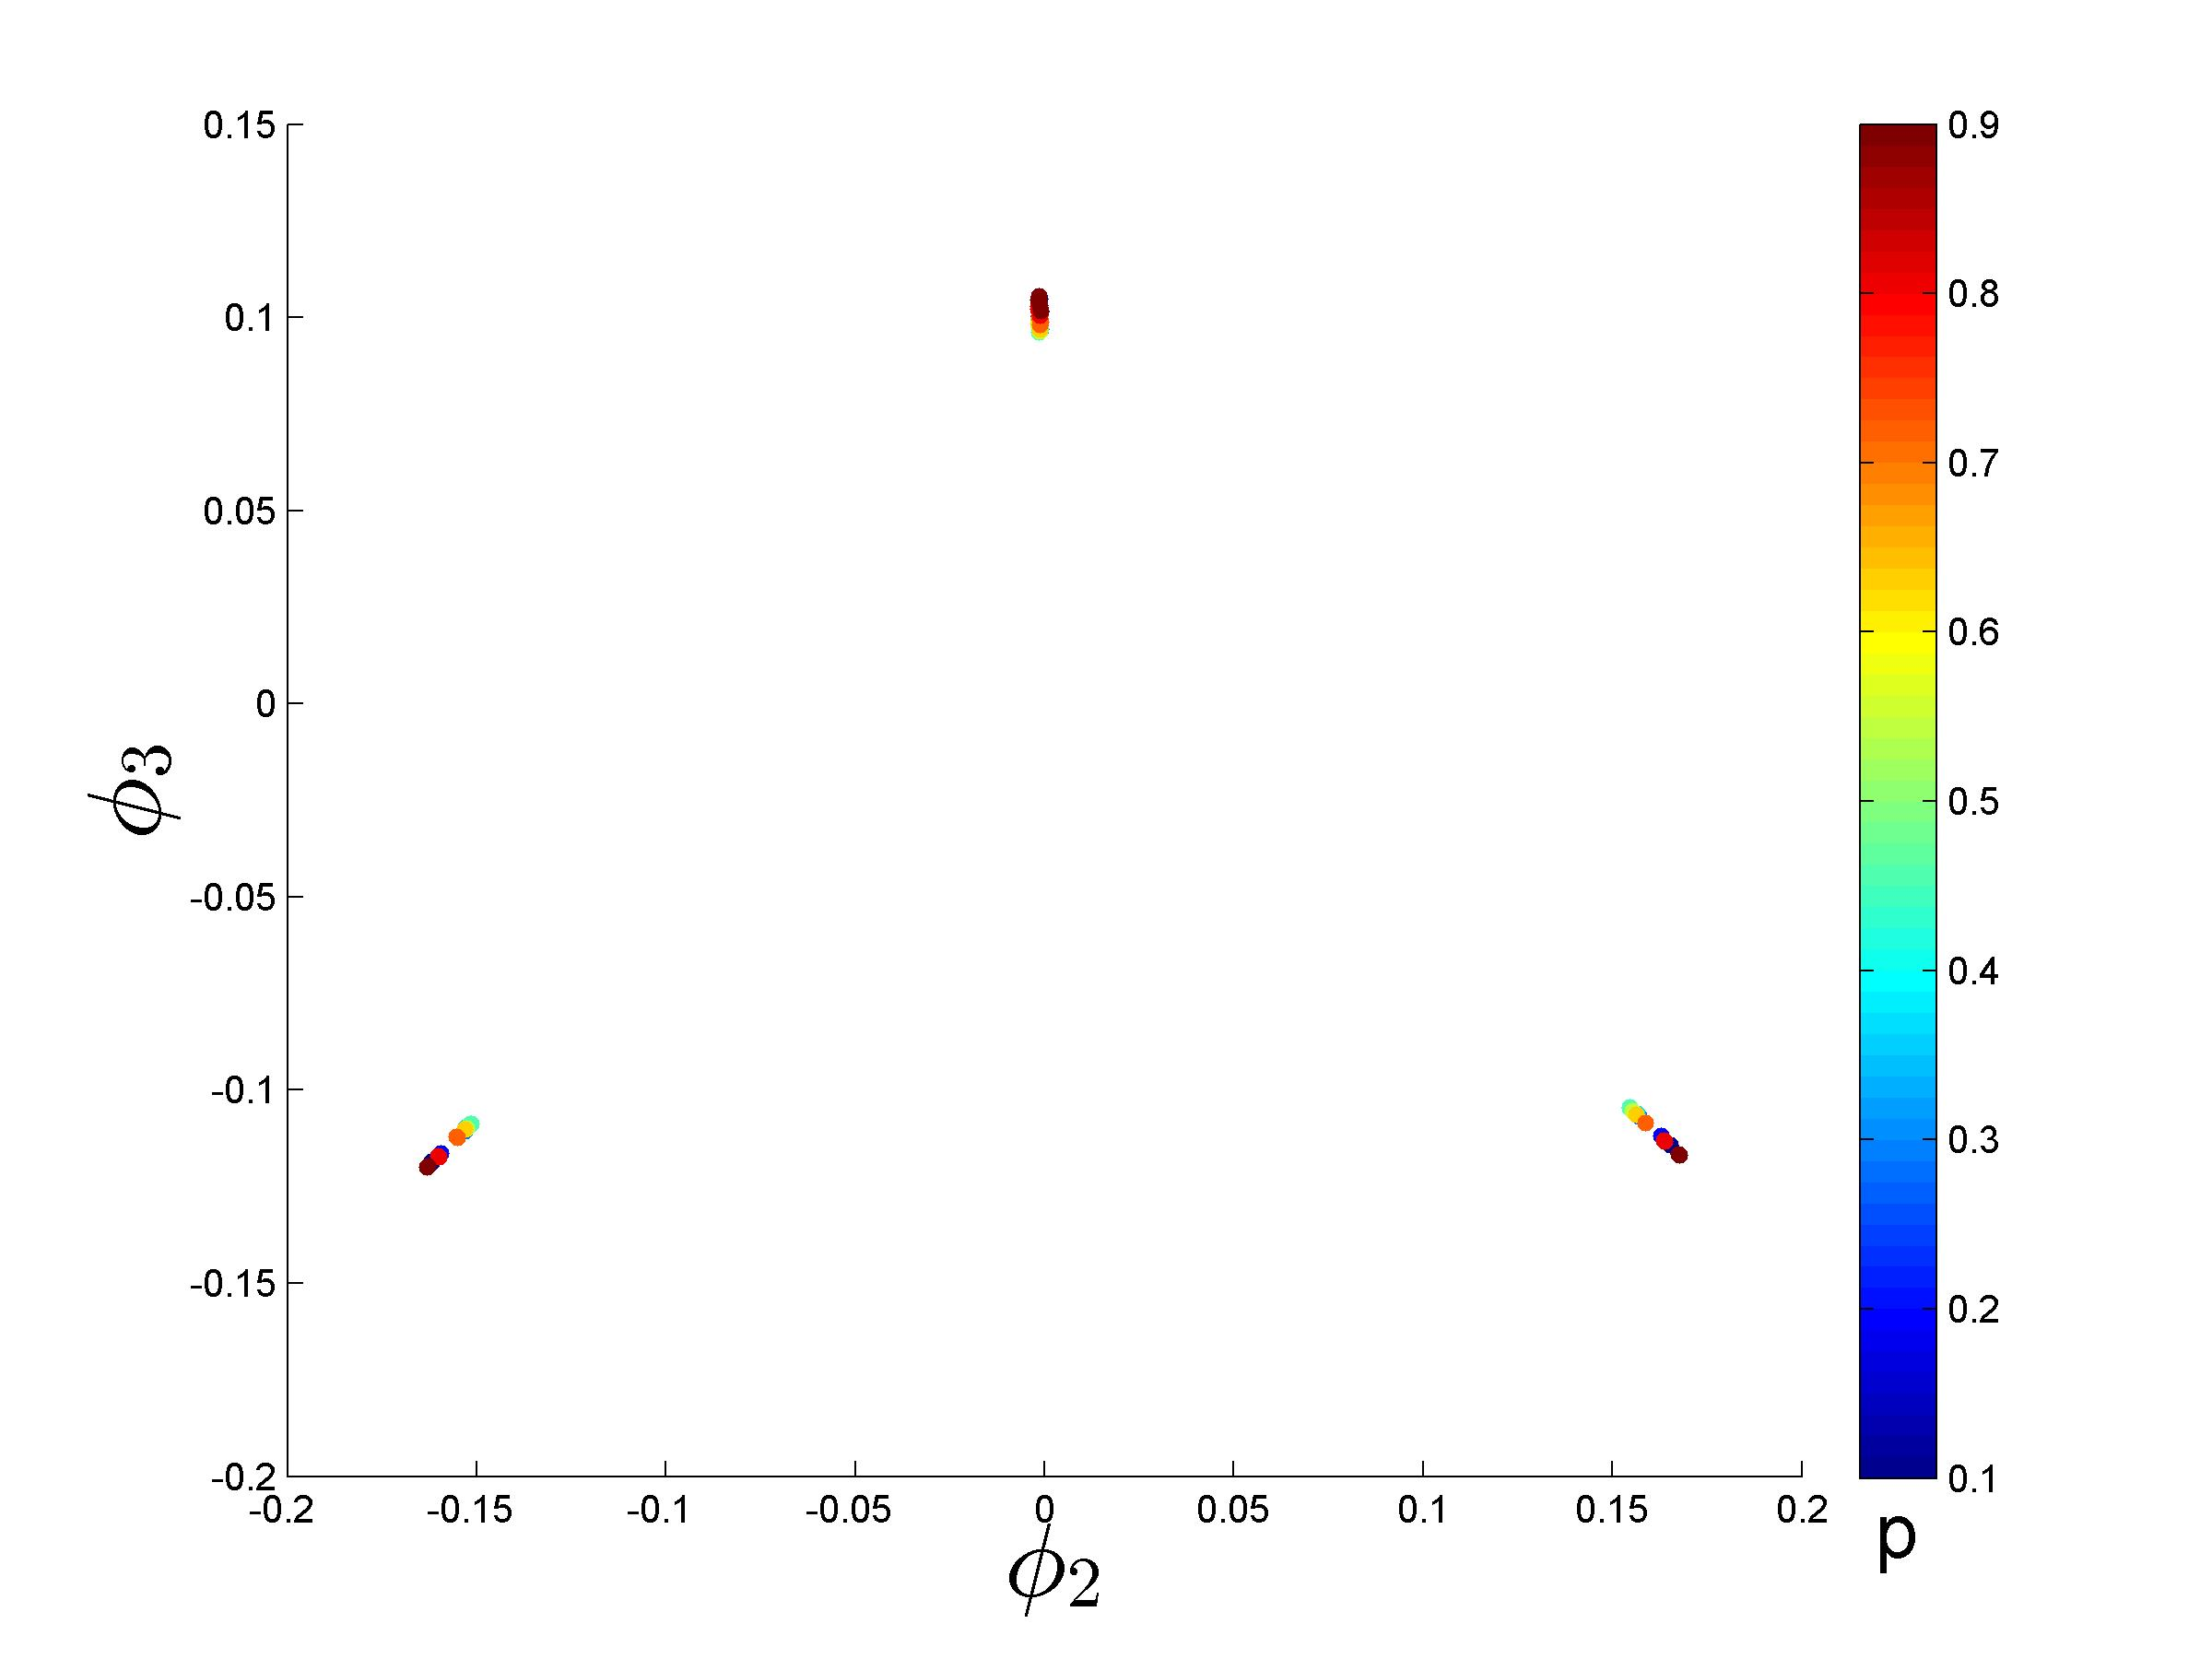
\includegraphics[width=\textwidth]{rawhist_p_1}
\caption{}
\end{subfigure}
\begin{subfigure}{0.2\textwidth}
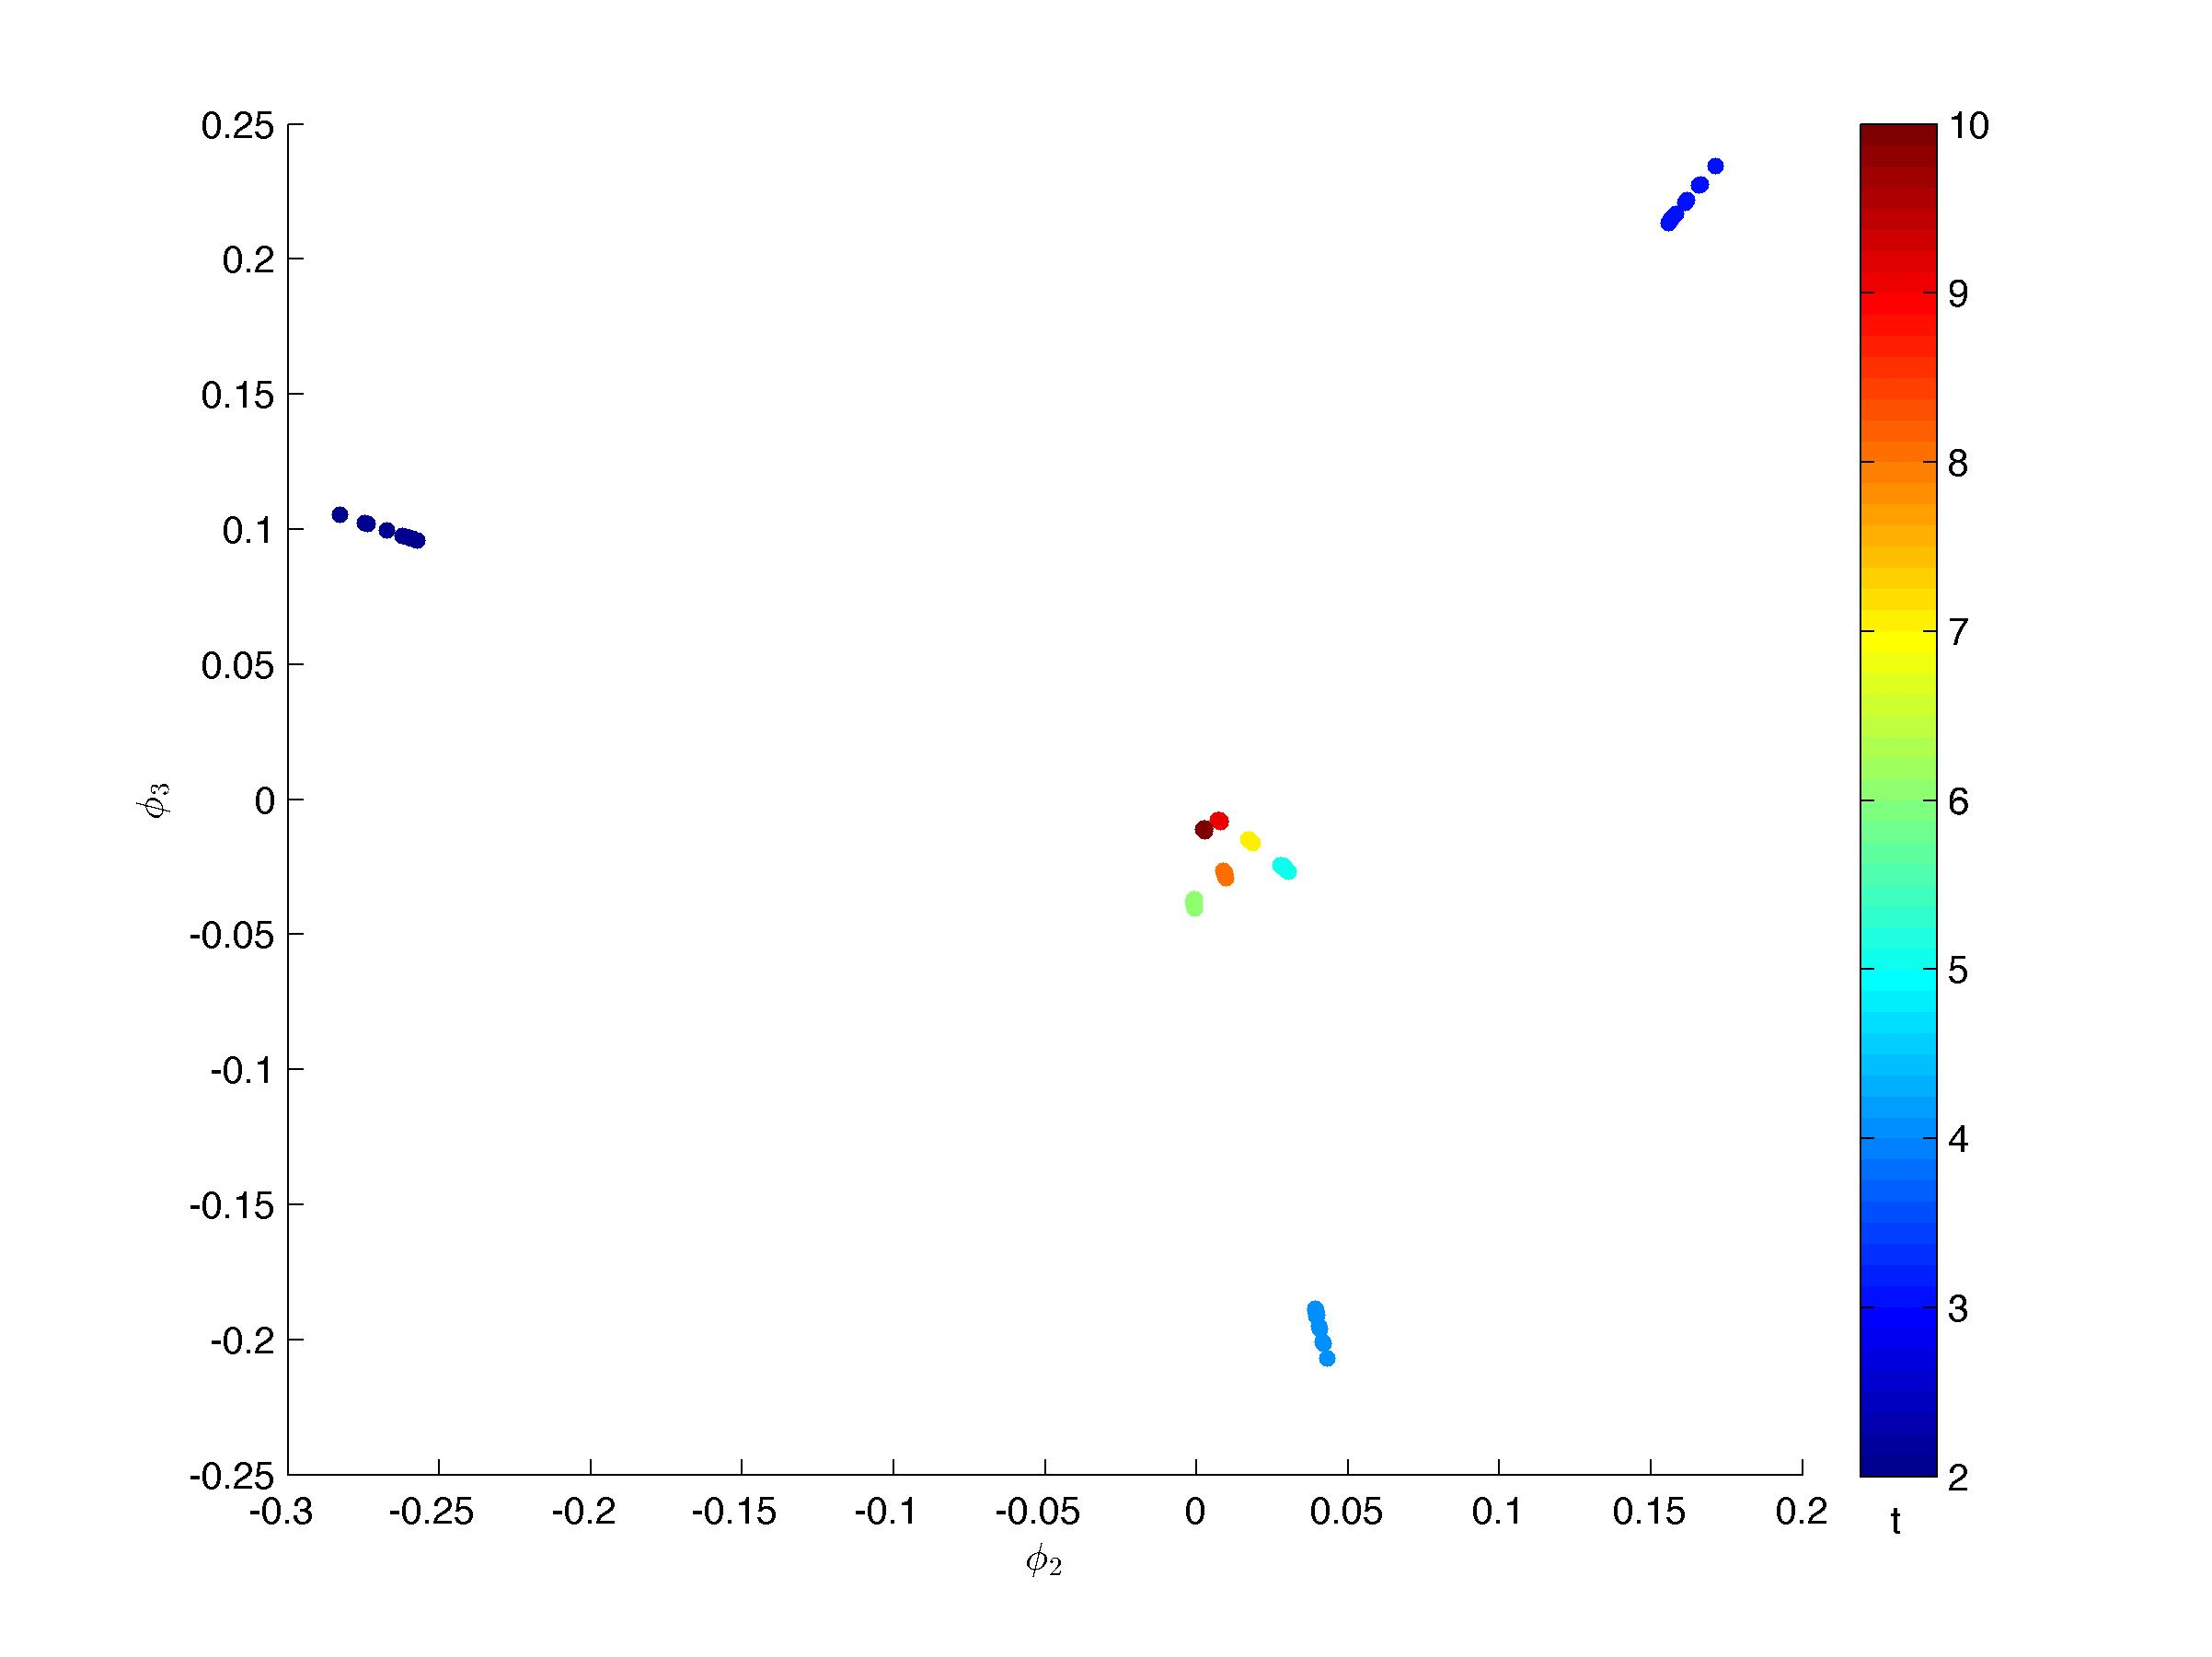
\includegraphics[width=\textwidth]{rawhist_t_1}
\caption{}
\end{subfigure}
\begin{subfigure}{0.2\textwidth}
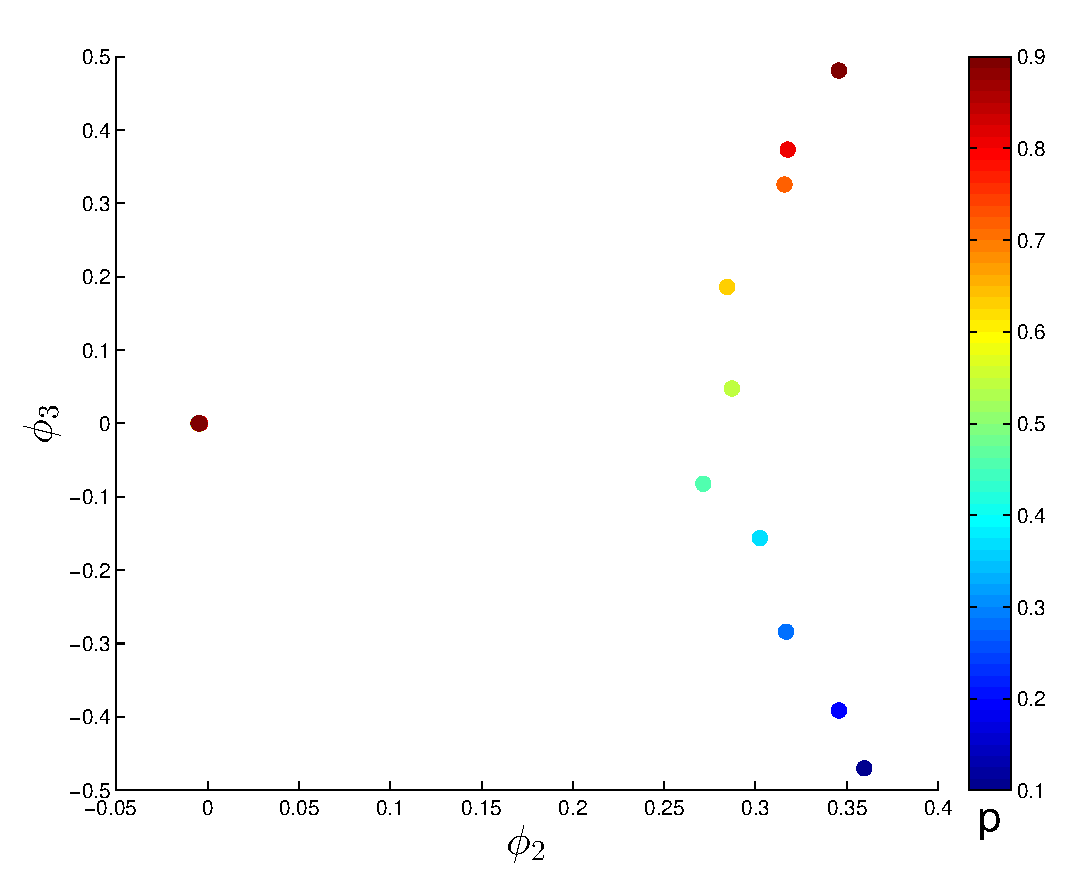
\includegraphics[width=\textwidth]{rawhist_p_400}
\caption{}
\end{subfigure}
\begin{subfigure}{0.2\textwidth}
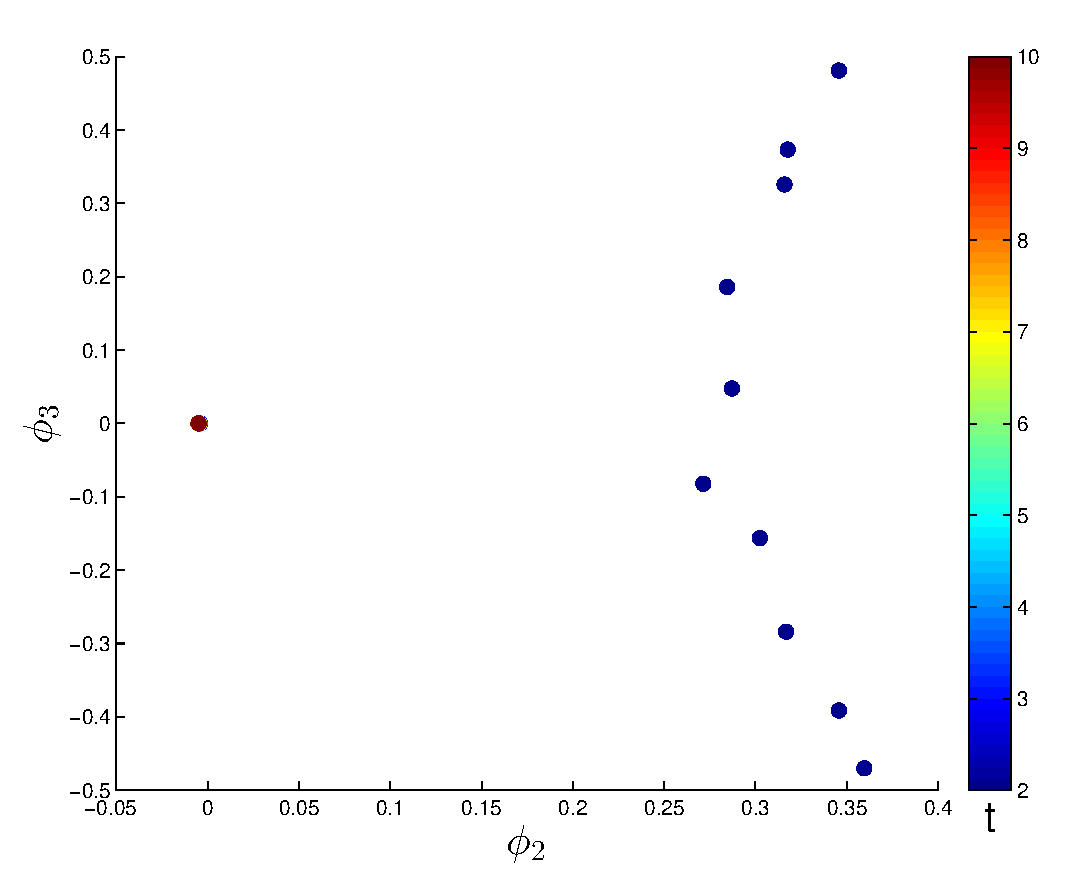
\includegraphics[width=\textwidth]{rawhist_t_400}
\caption{}
\end{subfigure}
\caption{Diffusion maps embeddings computed from simulation data of the velocity jump process with (a,b) $\lambda=1$, $s=1$, and (c,d) $\lambda=400$, $s=20$. The distances used in the diffusion maps kernel are the Euclidean distances between the histograms of particle positions. The data are colored by (a, c) $p$, the initial probability of left--moving particles, and (b, d) $t$, time. The first two diffusion maps modes do not accurately capture the important parameters in our simulations.}
\label{fig:dmaps_embed_noemd}
\end{figure*}

\begin{figure*}[htb]
\begin{subfigure}{0.4\textwidth}
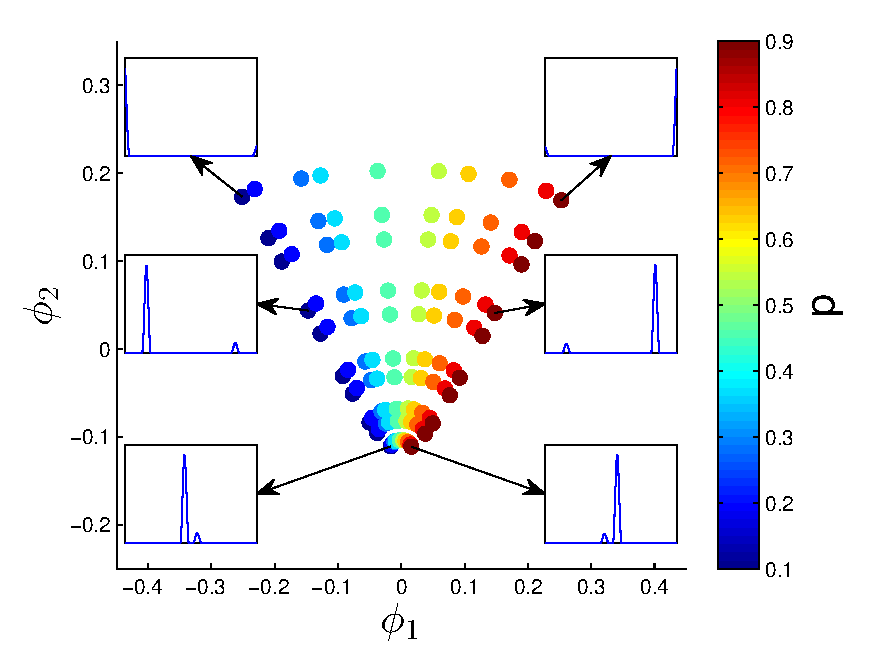
\includegraphics[width=\textwidth]{EMD_withhist_p_1}
\caption{}
\end{subfigure}
\begin{subfigure}{0.4\textwidth}
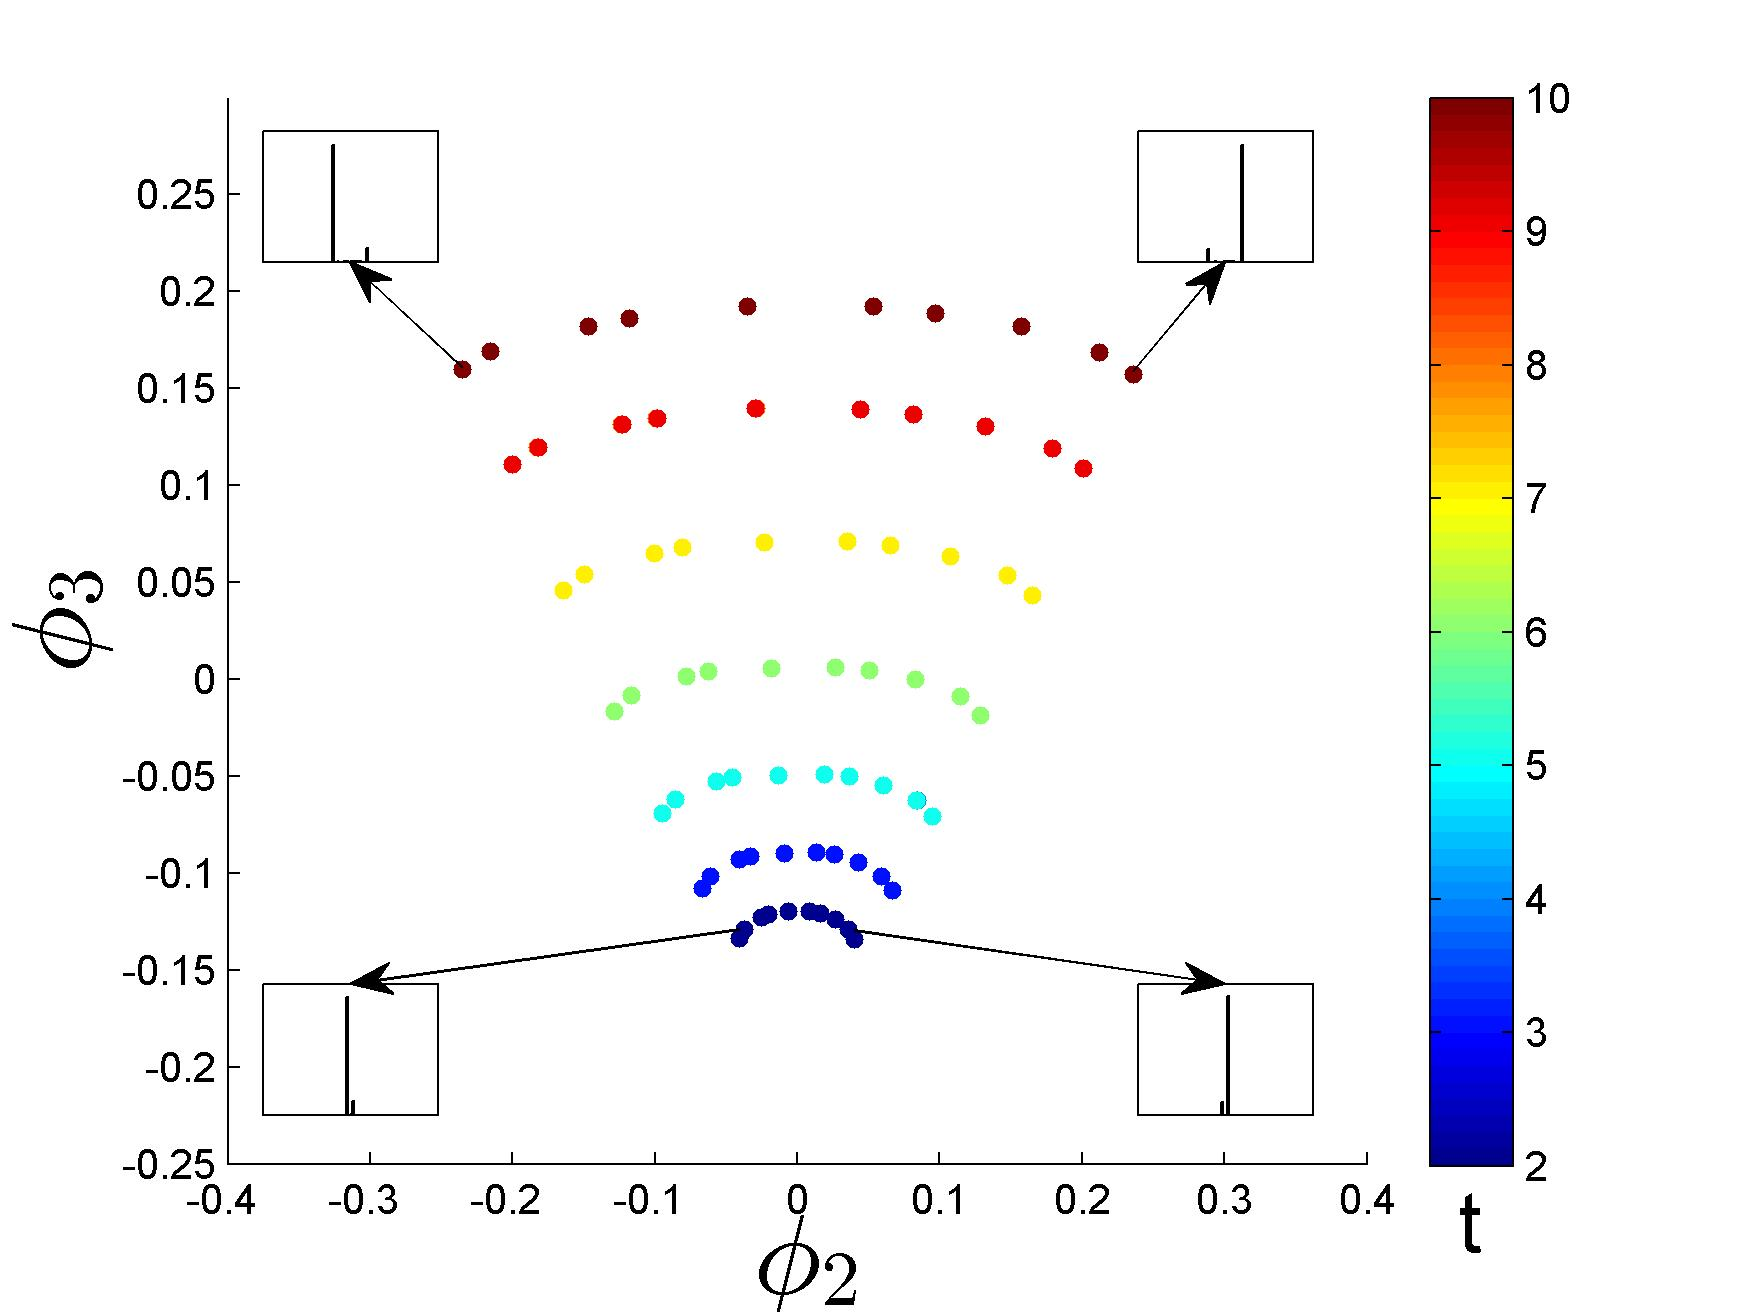
\includegraphics[width=\textwidth]{EMD_withhist_t_1}
\caption{}
\end{subfigure}
\begin{subfigure}{0.4\textwidth}
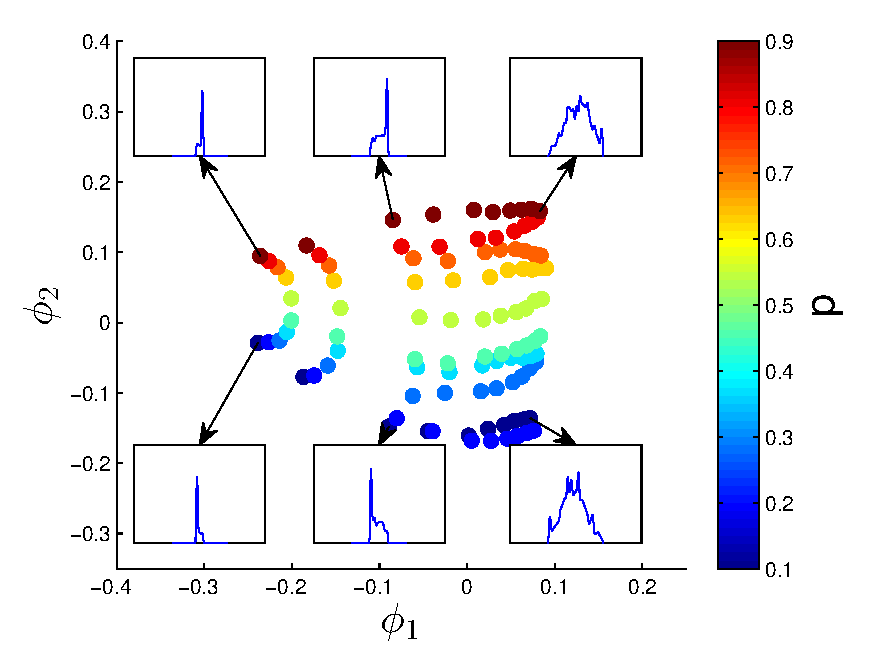
\includegraphics[width=\textwidth]{EMD_withhist_p_400}
\caption{}
\end{subfigure}
\begin{subfigure}{0.4\textwidth}
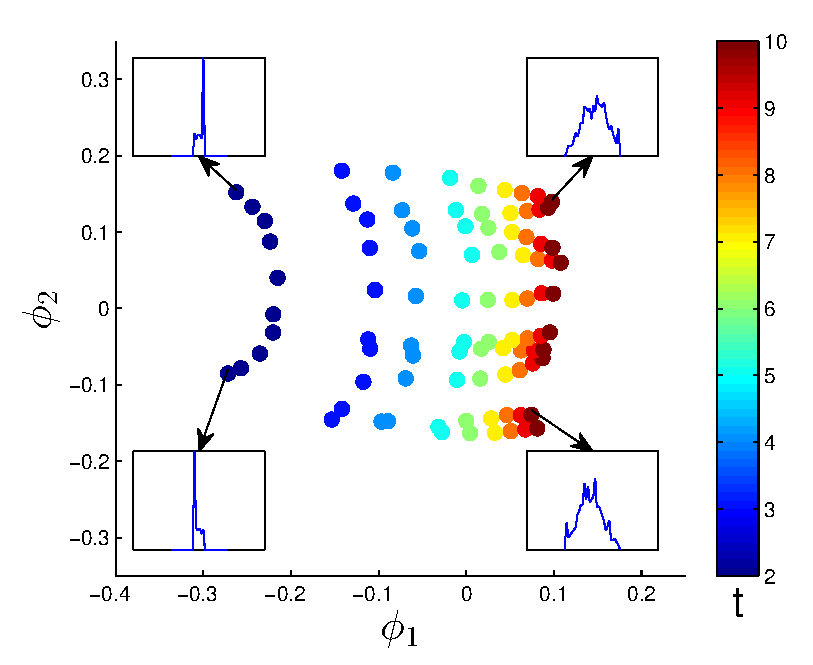
\includegraphics[width=\textwidth]{EMD_withhist_t_400}
\caption{}
\end{subfigure}
\caption{Diffusion maps embeddings computed from simulation data of the velocity jump process with (a,b) $\lambda=1$, $s=1$, and (c,d) $\lambda=400$, $s=20$. The distances used in the diffusion maps kernel are the earth mover's distances between the histograms of particle positions. The data are colored by (a, c) $p$, the initial probability of left--moving particles, and (b, d) $t$, time. }
\label{fig:dmaps_embed_emd}
\end{figure*}

\section{Discussion}


\bibliography{../../references/references}

\end{document}